\chapter[\label{c:intro}\protect\vspace{-1.3ex}Introduction: This Chapter Title
is Very Long, so we Can See\\ if a fancy trick makes it
single-spaced]{Introduction: This Chapter Title is Very Long, so we Can See if
a fancy trick makes it single-spaced}

\section{Welcome to my World}

See Appendix~\ref{a:hints} for some latex hints.  It's a good idea for
you to read them before you do anything else.  Then return here to see
how this content was done \dots


\subsection{What's Mine is Yours}

Lorem ipsum dolor sit amet, consectetur adipisicing elit, sed do eiusmod tempor incididunt ut labore et dolore magna aliqua. Ut enim ad minim veniam,

\subsection{What's Yours is Mine}


quis nostrud exercitation ullamco laboris nisi ut aliquip ex ea commodo consequat. Duis aute irure dolor in reprehenderit in voluptate velit esse



\subsection{What's Ours is is Theirs}

quis nostrud exercitation ullamco laboris nisi ut aliquip ex ea commodo consequat. Duis aute irure dolor in reprehenderit in voluptate velit esse
cillum dolore eu fugiat nulla pariatur. Excepteur sint occaecat cupidatat non proident, sunt in culpa qui officia deserunt mollit anim id est
laborum.

\subsubsection{Ownership is Theft (title should not be in TOC)}

Lorem ipsum dolor sit amet, consectetur adipisicing elit, sed do eiusmod tempor incididunt ut labore et dolore magna aliqua. Ut enim ad minim veniam,
est laborum.


%\addtocontents{toc}{\singlespacing}

\section{This is a Very Long Section Title, designed to show that it is double
space in table of contents unless the fancy trick is used}

laborum. Lorem ipsum dolor sit amet, consectetur adipisicing elit, sed do eiusmod tempor incididunt ut labore et dolore magna aliqua. Ut enim ad

%\addtocontents{toc}{\doublespacing}

est laborum. Lorem ipsum dolor sit amet, consectetur adipisicing elit, sed do eiusmod tempor incididunt ut labore et dolore magna aliqua. Ut enim ad
est laborum.


quis nostrud exercitation ullamco laboris nisi ut aliquip ex ea commodo consequat. Duis aute irure dolor in reprehenderit in voluptate velit esse
cillum dolore eu fugiat nulla pariatur. Excepteur sint occaecat cupidatat non proident, sunt in culpa qui officia deserunt mollit anim id est




\begin{equation}
	\label{e:expansion}
	\alpha = -\frac{1}{\rho}\frac{\partial \rho}{\partial T}
\end{equation}

Lord Rayleigh might have been the first to use \eqref{e:expansion}, but he surely wasn't the last. The equation comes up in
convection problems. Heated soup sometimes cools in spots, for a while, as convection cells roll over a sensor
(Figure~\ref{f:wigglyline}).  Some soups are yucky no matter the temperature (Table~\ref{t:soup}).

Literature citations can be done as ... ``\cite{Voss:2001} showed that (stuff)'' or 
``stuff \cite[]{Voss:2001}''.  To test the bib page, we'd
better cite some more, e.g. \cite{Baines:1973}, \cite{Baines:1982},
\cite{ostlund1981tldr}, 
\cite{boer1994raia},

\begin{figure}[htbp]
	\begin{center}
		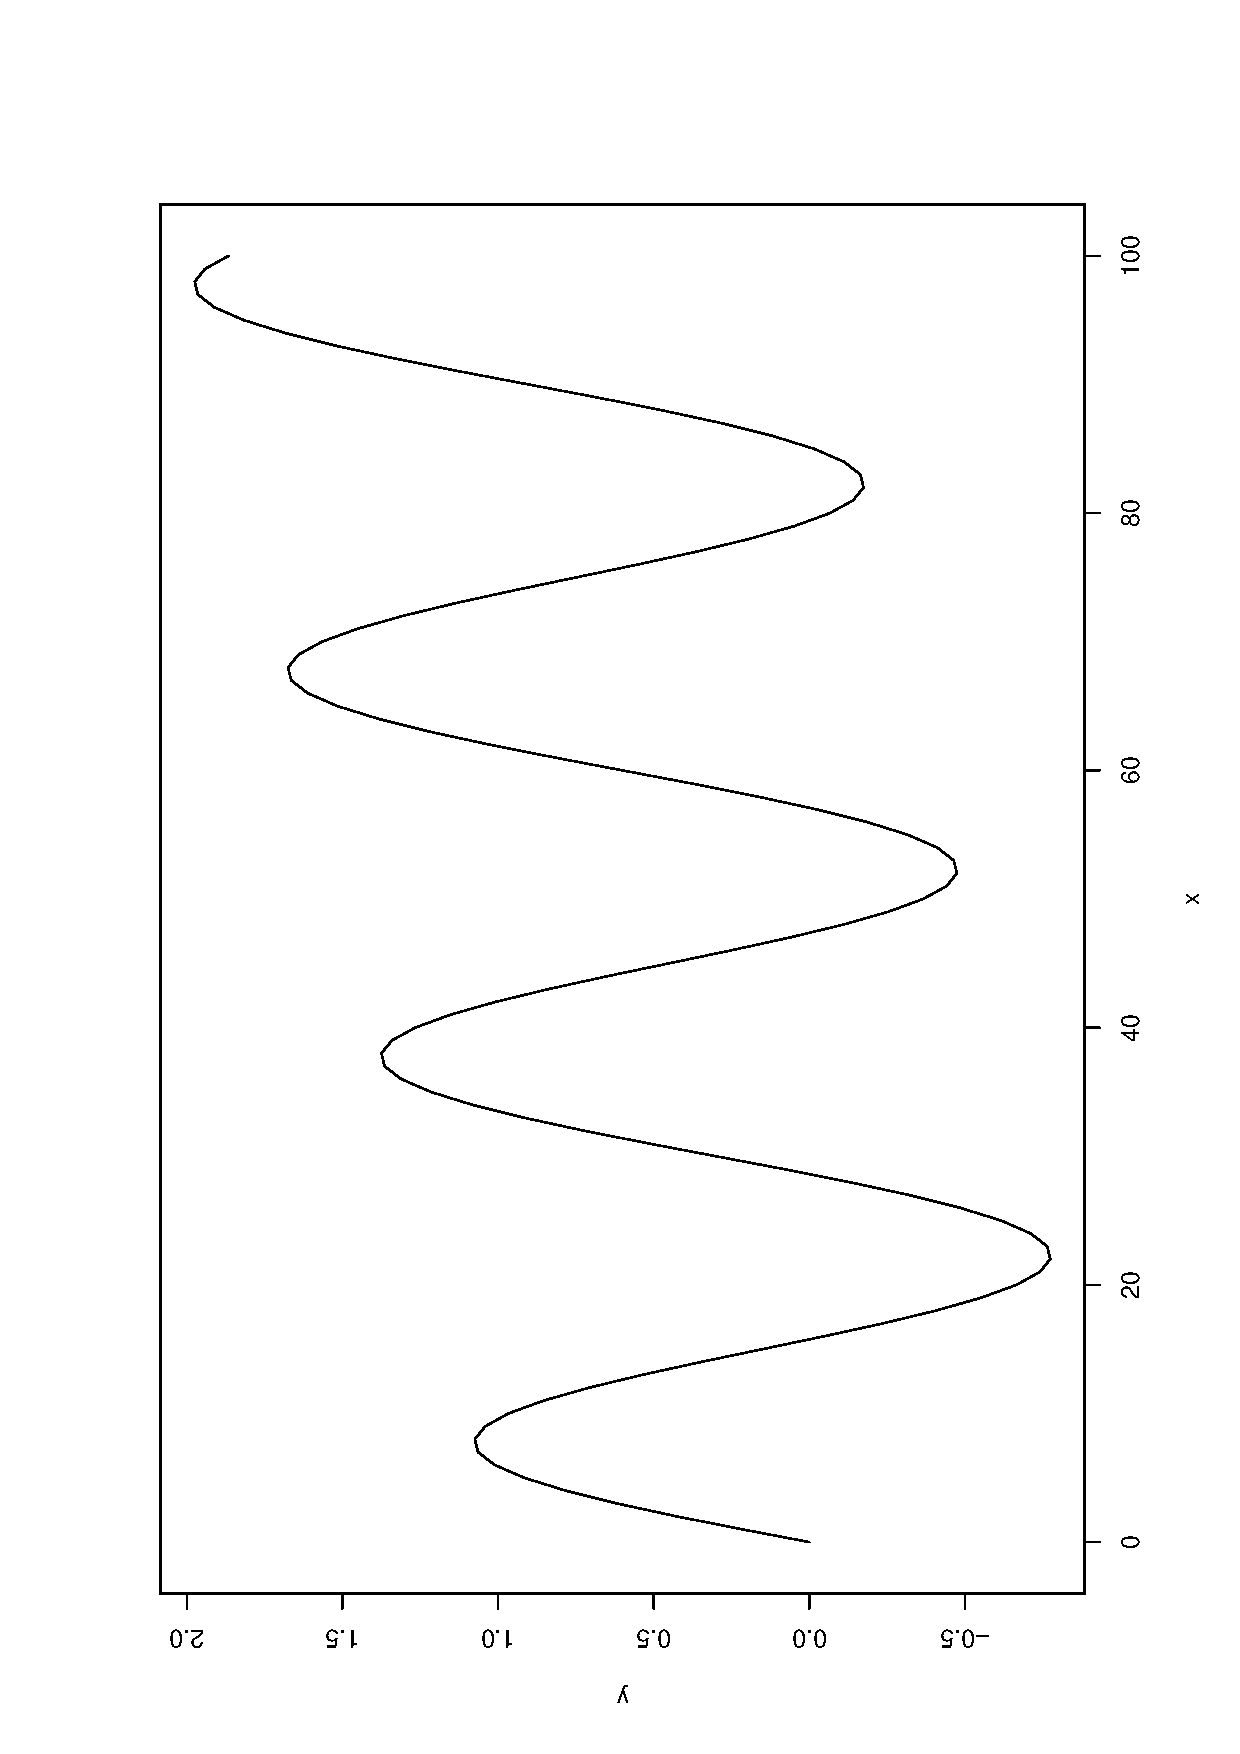
\includegraphics[scale=1]{figure1} % ask yourself what suffix is being used ...
	\end{center}
	\caption[Normalized temperature rise in heated soup]{
	\label{f:wigglyline}
	Oh Alabama./
	Can I see you /
	and shake your hand. /
	Make friends down in Alabama. /
	I'm from a new land /
	I come to you /
	and see all this ruin /
	What are you doing Alabama? /
	You got the rest of the union /
	to help you along /
	What's going wrong?  (\emph{Neil Young})}
\end{figure}

\begin{table}
  \begin{center}
    \begin{tabular}{|l|l|}
      \hline
      Soup  & Impression\\
      \hline
      Pea  & yummy in my tummy\\
      Carrot & not to my taste\\
      \hline
    \end{tabular}
  \end{center}
  \caption[Food for thought]{\label{t:soup}  Rows and flows of angel hair /and ice cream castles in the air / and feather canyons everywhere / I've looked at clouds that way. (\emph{Joni Mitchell})}
\end{table}


\section{Later skater}

\subsection{See ya later alligator}
\subsection{After a while crocodile}

\section{Goodbye}
%\layout

Lorem ipsum dolor sit amet, consectetur adipisicing elit, sed do
eiusmod tempor incididunt ut labore et dolore magna aliqua. Ut enim ad
minim veniam, quis nostrud exercitation ullamco laboris nisi ut
aliquip ex ea commodo consequat. Duis aute irure dolor in
reprehenderit in voluptate velit esse cillum dolore eu fugiat nulla
pariatur. Excepteur sint occaecat cupidatat non proident, sunt in
culpa qui officia deserunt mollit anim id est laborum.


